\documentclass[12pt,titlepage]{article}





%PACKAGES
\usepackage[ngerman]{babel}
\usepackage[utf8]{inputenc}
\usepackage[a4paper,lmargin={2.5cm},rmargin={2.5cm},
tmargin={2.5cm},bmargin = {2.5cm}]{geometry}
\usepackage{graphicx}
\usepackage{caption}
\usepackage{float}
\usepackage{hyperref}
\parindent0pt



\begin{document}



\thispagestyle{empty}

%TITELSEITE
\begin{center}
\textbf{Hochschule Luzern}\\
Departement für Informatik\\[12\baselineskip]

\begin{Huge}
PCP Projekt - Programmiersprachanalyse
\end{Huge} \\[6\baselineskip]

\begin{large}
\textbf{Analyse der Programmiersprache GO}
\end{large} \\[6\baselineskip]

\begin{large}
\textbf{Studierende}: Frederico Fischer, Oliver Werlen\\
\textbf{Dozenten}: Prof. Dr. Ruedi Arnold, Marcel Baumann \\

\textbf{Abgabedatum}: 26. Mai 2021 \\
\end{large}
\end{center}
\newpage


\section{Einleitung}

\section{Vision, Geschichte \& Verbreitung}

\section{Sprachkonstrukte}
    
\subsection{Goroutines, Channels \& Select}
\subsubsection{Goroutines}
Eine Goroutine ist ein leichtgewichtiger Thread, welcher von der Go runtime gemanaged wird. Goroutines nutzen dabei den selben Adressraum, daher muss der Zugriff auf geteilte Ressourcen synchronisiert werden. In Go gibt es Primitives, welche die Synchronisierung übernehmen. Jedoch werden diese nur selten genutzt, da in den meisten Fällen mit Channels gearbeitet wird. 
\subsubsection{Channels}
Ein Channel erlaubt einen einfachen Datenfluss. Per Default ist dabei das Senden und Empfangen blockierend, bis die andere Seite bereit ist. Goroutines lassen sich somit sehr leicht synchronisieren, ohne den Einsatz von Locks oder Variablen. Der Channel kann explizit vom Sender geschlossen werden. Damit wird dem Empfänger signalisiert, dass keine Werte mehr empfangen werden können. Das Schliessen des Channels sollte dabei exklusiv vom Sender ausgeführt werden. Senden auf einen geschlossenen Channel verursacht dabei "panic".

\subsubsection{Select}
Bei einem Select wird bei mehrfacher Auswahl gewartet, bis eine Operation laufen kann. 

\subsubsection{Beispiel}
Im Beispiel unten werden alle oben genannten Sprachkonstrukte genutzt. Bei func() handelt es sich um eine Goroutine, welche 10 Werte von dem Channel c liesst und anschliessend einen Wert auf den Quit-Channel schreibt. Das Select diffenziert dabei zwischen den beiden Channels. Je nach Case wird entweder eine neue Fibonacci-Zahl berechnet oder der Channel geschlossen. 
\begin{figure}[H]
	\centering
	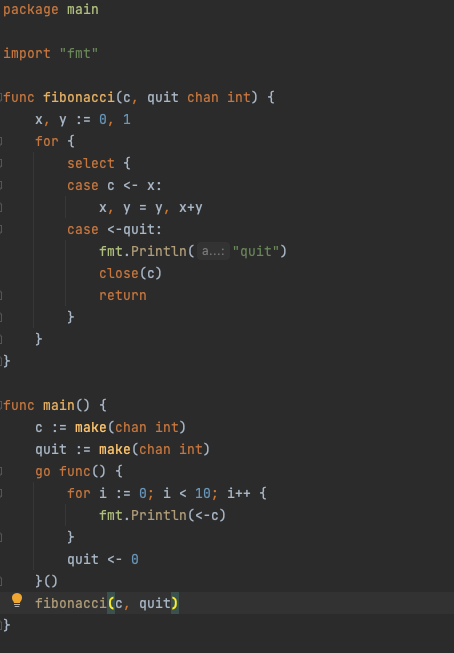
\includegraphics[scale=0.3]{fibGoroutine.PNG}
	\caption[Beispiel Goroutine, Channel und Select]{Beispiel Goroutine, Channel und Select,\\ Quelle: Autor}
	\label{img: fibGoroutine}
\end{figure} 


\subsection{Maps \& Slices}
Erklärung und Codebeispiel


\subsection{Structural \& Nominal Typing}
Erklärung und Codebeispiel


\subsection{The Go Memory Model}
Erklärung und Codebeispiel


\subsection{Package Management}
Erklärung und Codebeispiel


\subsection{Defer}
Erklärung und Codebeispiel

\section{Fazit}
\subsection{Team-Fazit}

\subsection{Fazit Frederico Fischer}

\subsection{Fazit Oliver Werlen}

    

\end{document}